\section{General Wiring}
The setup is wired as described in figure \ref{fig:wiring}.
\begin{figure}[htbp]
\centering
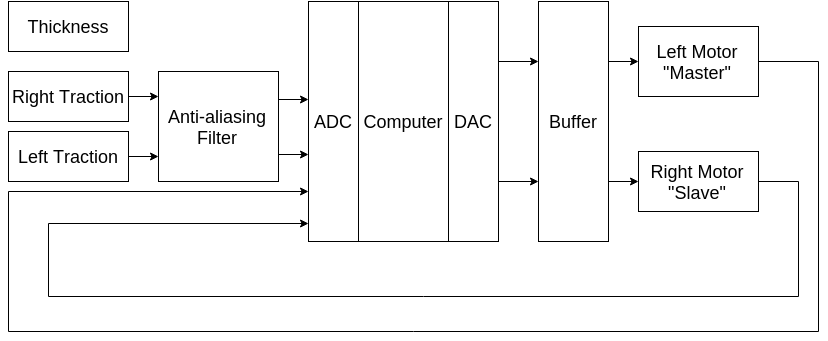
\includegraphics[width = \textwidth]{wiring.png}
\caption{\label{fig:wiring}Wiring for the control of the rolling mill}
\end{figure}
We use the maximum recommended sampling frequency $f_s  = \SI{100}{\hertz}$, which is a common value for the control of a DC motor.

\subsection{Anti-aliasing filtering}
To be perfectly rigorous, we should filter every input before sampling it. However, we only have a limited amount of single signal, second order Butterworth filters at our disposition, each with a different $f_c$. With the chosen $f_s$, those constraints on the available $f_c$, and the fact that second order Butterworth filters have a large transition band, only two of the available $f_c$ values seem actually useful:
\begin{itemize}
 \item $f_c = \SI{40}{\hertz}$, which provides \SI{37.1}{\percent} attenuation at \SI{50}{\hertz} and \SI{62.9}{\percent} rejection at \SI{100}{\hertz}.
 \item $f_c = \SI{20}{\hertz}$, which provides \SI{62.9}{\percent} attenuation at \SI{50}{\hertz} and \SI{80.4}{\percent} rejection at \SI{100}{\hertz}.
\end{itemize}

The other available filters either do not actually prevent aliasing, or have a too high passband attenuation. Even the two most adequate filters have a non ideal passband gain, and thus introduce a significant delay in the feedback loop. For this reason we choose not to use them in the inner loop, which should be fast, but rather in the outer loop. This is why only the two traction measurements are filtered in figure \ref{fig:wiring}.
